% \pagebreak[4]
% \hspace*{1cm}
% \pagebreak[4]
% \hspace*{1cm}
% \pagebreak[4]

\chapter{Giới thiệu }
\ifpdf
    \graphicspath{{Chapter1/Chapter1Figs/PNG/}{Chapter1/Chapter1Figs/PDF/}{Chapter1/Chapter1Figs/}}
\else
    \graphicspath{{Chapter1/Chapter1Figs/EPS/}{Chapter1/Chapter1Figs/}}
\fi

Nhờ vào những cải cách trong giao thông và cơ sở hạ tầng viễn thông mà giờ đây toàn cầu hóa đang trở nên gần với chúng ta hơn bao giờ hết. Trong xu hướng đó nhu cầu giao tiếp và thông hiểu giữa những nền văn hóa là không thể thiếu. Tuy nhiên, những nền văn hóa khác nhau thường kèm theo đó là sự khác biệt về ngôn ngữ, là một trong những trở ngại lớn nhất của sự giao tiếp. Một người phải mất rất nhiều thời gian để thành thạo một ngôn ngữ không phải là tiếng mẹ đẻ, và không thể nào học được nhiều ngôn ngữ cùng lúc. Cho nên, việc phát triển một công cụ để giải quyết vấn đề này là tất yếu. Một trong những công cụ như vậy là \textit{Dịch máy}.

\textit{Dịch máy} là quá trình chuyển đổi văn bản/tiếng nói từ ngôn ngữ này sang dạng tương ứng của nó trong một ngôn ngữ khác, được thực hiện bởi một chương trình máy tính nhằm mục đích cung cấp bản dịch tốt nhất mà không cần sự trợ giúp của con người. Trong khóa luận này, chúng tôi tập trung nghiên cứu dịch máy trên dữ liệu văn bản.

Dịch máy có một quá trình lịch sử lâu dài. Từ thế kỷ XVII, đã có những ý tưởng về việc cơ giới hóa quá trình dịch thuật. Tuy nhiên, đến thế kỷ XX, những nghiên cứu về dịch máy mới thật sự bắt đầu. Vào những năm 1930, Georges Artsrouni người Pháp và Petr Troyanskii người Nga đã nộp bằng sáng chế cho công trình có tên "máy dịch" của riêng họ. Trong số hai người, công trình của Troyanskii có ý nghĩa hơn. Nó đề xuất không chỉ một phương pháp cho bộ từ điển tự động, mà còn là lược đồ cho việc mã hóa các vai trò ngữ pháp song ngữ và một phác thảo về cách phân tích và tổng hợp có thể hoạt động. Tuy nhiên, những ý tưởng của Troyanskii đã không được biết đến cho đến cuối những năm 1950. Trước đó, máy tính đã được phát minh.

Những nỗ lực xây dựng hệ thống dịch máy bắt đầu ngay sau khi máy tính ra đời. Có thể nói, chiến tranh và sự thù địch giữa các quốc gia là động lực lớn nhất cho dịch máy thời bấy giờ. Trong Thế chiến thứ II, máy tính đã được quân đội Anh sử dụng trong việc giải mã các thông điệp được mã hóa của quân Đức. Việc làm này có thể coi là một dạng của dịch máy khi người ta cố gắng dịch từ tiếng Đức được mã hóa sang tiếng Anh. Trong thời kỳ chiến tranh lạnh, vào tháng 7/1949, Warren Weaver, người được xem là nhà tiên phong trong lĩnh vực dịch máy, đã viết một bản ghi nhớ (memorandum) đưa ra các đề xuất khác nhau của ông trong lĩnh vực này \cite{hutchins}. Những đề xuất đó dựa trên thành công của máy phá mã, sự phát triển của lý thuyết thông tin bởi Claude Shannon và suy đoán về các nguyên tắc phổ quát cơ bản của ngôn ngữ. Trong vòng một năm, một vài nghiên cứu về dịch máy đã bắt đầu tại nhiều trường đại học của Mỹ. Vào ngày 7/1/1954, tại trụ sở chính của IBM ở New York, thử nghiệm Georgetown-IBM được tiến hành. Máy tính IBM 701 đã tự động dịch 49 câu tiếng Nga sang tiếng Anh lần đầu tiên trong lịch sử chỉ sử dụng 250 từ vựng và sáu luật ngữ pháp \cite{hutchins}. Thí nghiệm này được xem như là một thành công và mở ra kỉ nguyên cho những nghiên cứu với kinh phí lớn về dịch máy ở Hoa Kỳ. Ở Liên Xô những thí nghiệm tương tự cũng được thực hiện không lâu sau đó.

Trong một thập kỷ tiếp theo, nhiều nhóm nghiên cứu về dịch máy được thành lập. Một số nhóm chấp nhận phương pháp thử và sai, thường dựa trên thống kê với mục tiêu là một hệ thống dịch máy có thể hoạt động ngay lập tức, tiêu biểu như: nhóm nghiên cứu tại đại học Washington (và sau này là IBM) với hệ thống dịch Nga-Anh cho Không quân Hoa Kỳ, những nghiên cứu tại viện Cơ học Chính xác ở Liên Xô và Phòng thí nghiệm Vật lý Quốc gia ở Anh. Trong khi một số khác hướng đến giải pháp lâu dài với hướng tiếp cận lý thuyết bao gồm cả những vấn đề liên quan đến ngôn ngữ cơ bản như nhóm nghiên cứu tại Trung tâm nghiên cứu lý thuyết tại MIT, Đại học Havard và Đơn vị nghiên cứu ngôn ngữ Đại học Cambridge. Những nghiên cứu trong giai đoạn này có tầm quan trọng và ảnh hưởng lâu dài không chỉ cho Dịch máy mà còn cho nhiều ngành khác như Ngôn ngữ học tính toán, Trí tuệ nhân tạo - cụ thể là việc phát triển các từ điển tự động và kỹ thuật phân tích cú pháp. Nhiều nhóm nghiên cứu đã đóng góp đáng kể cho việc phát triển lý thuyết ngôn ngữ. Tuy nhiên, mục tiêu cơ bản của dịch máy là xây dựng hệ thống có khả năng tạo ra bản dịch tốt lại không đạt được dẫn đến một kết quả là vào năm 1966, bản báo cáo từ Ủy ban tư vấn xử lý ngôn ngữ tự động (Automatic Language Processing Advisory) của Hoa Kỳ, tuyên bố rằng dịch máy là đắt tiền, không chính xác và không mang lại kết quả hứa hẹn \cite{hutchins}. Thay vào đó, họ đề nghị tập trung vào phát triển các từ điển, điều này đã loại bỏ các nhà nghiên cứu Mỹ ra khỏi cuộc đua trong gần một thập kỷ.

\begin{figure}
	\centering
	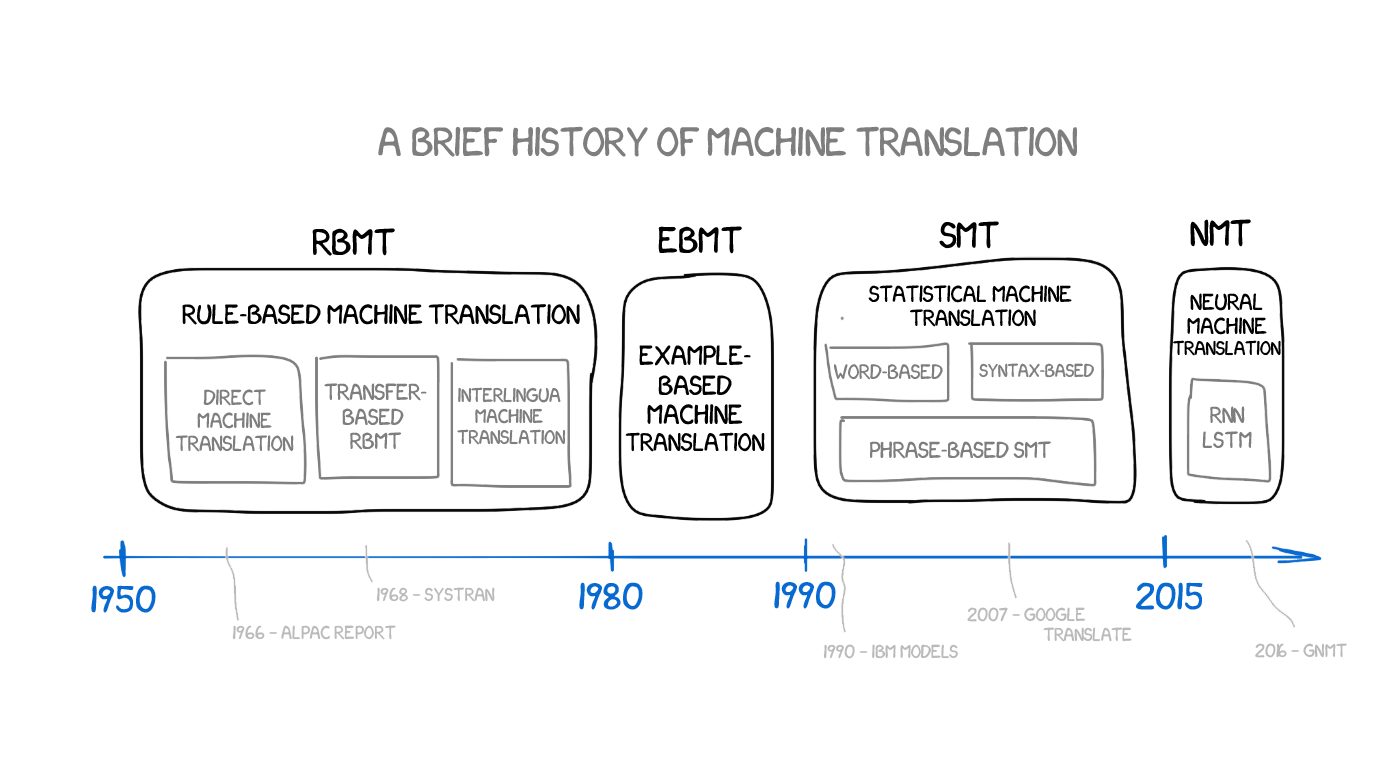
\includegraphics[width=\textwidth]{mthistory}
	\caption[Lịch sử tóm tắt của dịch máy]{Lịch sử tóm tắt của dịch máy, nguồn ảnh: Ilya Pestov trong blog \href{https://medium.freecodecamp.org/a-history-of-machine-translation-from-the-cold-war-to-deep-learning-f1d335ce8b5}{"A history of machine translation from the Cold War to deep learning"}}
	\label{fig_mthistory}
\end{figure}

Từ những năm 1950 đến nay, đã có nhiều hướng tiếp cập đã được sử dụng trong dịch máy với mục tiêu tạo ra bản dịch có độ chính xác cao và giảm thiểu công sức của con người. Hình \ref{fig_mthistory} thể hiện các phương pháp dịch máy đã được đề xuất trong quá trình hình thành và phát triển của dịch máy từ những năm 1950. Trong những năm đầu tiên, để tạo ra bản dịch tốt, các phương pháp thời bấy giờ đều đòi hỏi những lý thuyết tinh vi về ngôn ngữ học. Hầu hết những hệ thống dịch máy trước những năm 1980 đều là \textit{dịch máy dựa trên luật (rule-based machine translation)}. Những hệ thống này thường bao gồm:
\begin{itemize}
	\item[•] Một từ điển song ngữ (ví dụ từ điển Anh - Đức)
	\item[•] Một tập các luật ngữ pháp (ví dụ trong tiếng Đức, từ kết thúc bằng -heit, -keit, -ung là những từ mang giống cái)		
\end{itemize} 

\begin{figure}
	\centering
	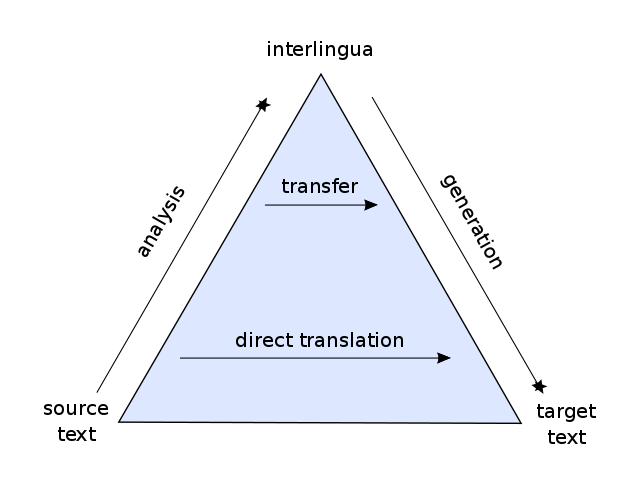
\includegraphics[width=0.5\textwidth]{rulebasedpyramid}
	\caption[Ba phương pháp dịch máy dựa trên luật]{Kim tự tháp của Bernard Vauquois thể hiện ba phương pháp dịch máy dựa luật theo độ sâu của đại diện trung gian. Bắt đầu từ dịch máy trực tiếp đến dịch máy chuyển dịch và trên cùng là dịch máy ngôn ngữ phổ quát (Nguồn: \href{http://en.wikipedia.org/wiki/Machine_translation}{http://en.wikipedia.org/wiki/Machine\_translation})}
	\label{fig_rulebasedpyramid}
\end{figure}

Có ba cách tiếp cận khác nhau theo phương pháp dịch máy dựa trên luật, bao gồm: dịch máy trực tiếp, dịch máy chuyển giao và dịch máy ngôn ngữ phổ quát. Mặc dù cả ba đều thuộc về dịch máy dựa trên luật, tuy nhiên chúng khác nhau về độ sâu của đại diện trung gian. Sự khác biệt này được thể hiện qua kim tự tháp Vauquois, minh họa trên hình \ref{fig_rulebasedpyramid}.

\textit{Dịch máy trực tiếp} (Direct machine translation): Đây là phương pháp đơn giản nhất của dịch máy. Dịch máy trực tiếp không dùng bất cứ dạng đại diện nào của ngôn ngữ nguồn, nó chia câu thành các từ, dịch chúng bằng một từ điển song ngữ. Sau đó, dựa trên các luật mà những nhà ngôn ngữ học đã xây dựng, nó chỉnh sửa để bản dịch trở nên đúng cú pháp và ít nhiều đúng về mặt phát âm.

\textit{Dịch máy ngôn ngữ phổ quát} (Interlingual machine translation): Trong phương pháp này, câu nguồn được chuyển thành biểu diễn trung gian và biểu diễn này được thống nhất cho tất cả ngôn ngữ trên thế giới (interlingua). Tiếp theo, dạng đại diện này sẽ được chuyển đổi sang bất kỳ ngôn ngữ đích nào. Một trong những ưu điểm chính của hệ thống này là tính mở rộng của nó khi số lượng ngôn ngữ cần dịch tăng lên. Mặc dù trên lý thuyết, phương pháp này trông rất hoàn hảo. Nhưng trong thực tế, thật khó để tạo được một ngôn ngữ phổ quát như vậy.

\textit{Dịch máy chuyển giao} (Transfer-based machine translation): dịch máy chuyển giao tương tự như dịch máy ngôn ngữ phổ quát ở chỗ, nó cũng tạo ra bản dịch từ biểu diễn trung gian mô phỏng ý nghĩa của câu gốc. Tuy nhiên, không giống như dịch máy ngôn ngữ phổ quát, dịch máy chuyển giao phụ thuộc một phần vào cặp ngôn ngữ mà nó tham gia vào quá trình dịch. Trên cơ sở sự khác biệt về cấu trúc của ngôn ngữ nguồn và ngôn ngữ đích, một hệ thống dịch máy chuyển giao có thể được chia thành ba giai đoạn: i) Phân tích, ii) Chuyển giao, iii) Tạo ra bản dịch. Trong giai đoạn đầu tiên, trình phân tích cú pháp ở ngôn ngữ nguồn được sử dụng để tạo ra biểu diễn cú pháp của câu nguồn. Trong giai đoạn tiếp theo, kết quả của phân tích cú pháp được chuyển đổi thành biểu diễn tương đương trong ngôn ngữ đích. Trong giai đoạn cuối cùng, một bộ phân tích hình thái của ngôn ngữ đích được sử dụng để tạo ra các bản dịch cuối cùng.

Mặc dù đã có một số hệ thống dịch máy dựa trên luật được đưa vào sử dụng như PROMPT (\url{http://www.promt.com/}) và Systrans (\url{http://www.systransoft.com/}). Tuy nhiên, bản dịch của hướng tiếp cận này có chất lượng thấp so với nhu cầu của con người và không sử dụng được trừ một số trường hợp đặc biệt. Ngoài ra chúng còn có một số nhược điểm lớn như:
\begin{itemize}
	\item[•] Các loại từ điển chất lượng tốt có sẵn là không nhiều và việc xây dựng những bộ từ điển mới là rất tốn kém.
	\item[•] Hầu hết những luật ngôn ngữ được tạo ra bằng tay bởi các nhà ngôn ngữ học. Việc này gây khó khăn và tốn kém khi hệ thống trở nên lớn hơn.
	\item[•] Các hệ thống dịch máy dựa trên luật gặp khó khăn trong việc giải quyết những vấn đề như thành ngữ hay sự nhập nhằng về ngữ nghĩa của các từ. 
\end{itemize}
Từ những năm 1980, dịch máy dựa trên \textit{Ngữ liệu} (Corpus-based machine translation) được đề xuất. Điểm khác biệt lớn nhất và cũng là quan trọng nhất của hướng tiếp cận này so với dịch máy dựa trên luật là thay vì sử dụng các bộ từ điển song ngữ, nó dùng những tập câu tương đương trong hai ngôn ngữ làm nền tảng cho việc dịch thuật. Tập những câu tương đương này được gọi là ngữ liệu. So với từ điển, việc thu thập ngữ liệu đơn giản hơn rất nhiều. Ví dụ như ta có thể tìm thấy nhiều phiên bản trong các ngôn ngữ khác nhau của những văn bản hành chính hay các trang web đa ngôn ngữ (hình \ref{fig_parallelcorpus} mô tả tập ngữ liệu Anh - Nga). Trước khi dịch máy nơ-ron ra đời, phương pháp dịch máy dựa trên ngữ liệu hiệu quả nhất chính là dịch máy thống kê.

\textit{Dịch máy thống kê} (Statistical machine translation): ý tưởng của phương pháp này là thay vì định nghĩa những từ điển và các luật ngữ pháp một cách thủ công, dịch máy thống kê dùng mô hình thống kê để học các từ điển và các luật ngữ pháp này từ ngữ liệu. Những ý tưởng đầu tiên của dịch máy thống kê được giới thiệu đầu tiên bởi Waren Weaver vào năm 1949 bap gồm việc áp dụng lý thuyết thông tin của Claude Shannon vào dịch máy. Dịch máy thống kê được giới thiệu lại vào cuối những năm 1980 và đầu những năm 1990 tại trung tâm nghiên cứu Thomas J. Watson của IBM. Dịch máy thống kê là phương pháp được nghiên cứu rộng rãi nhất thời bấy giờ và thậm chí đến hiện tại, nó vẫn là một trong những phương pháp được nghiên cứu nhiều nhất về dịch máy. 

Để hiểu rõ hơn về dịch máy thống kê, xét một ví dụ: ta cần dịch một câu $f$ trong tiếng Pháp sang dạng tiếng Anh $e$ của nó. Có nhiều bản dịch có thể có cuả $f$ trong tiếng Anh, việc cần làm là chọn $e$ sao cho nó là bản dịch "tốt nhất" của $f$. Chúng ta có thể mô hình hóa quá trình này bằng một xác suất có điều kiện $p(e|f)$ với $e$ là những bản dịch có thể có với câu cho trước $f$. Một cách hợp lý để chọn bản dịch "tốt nhất" là chọn $e$ sao cho nó tối đa xác suất có điều kiện $p(e|f)$. Cách tiếp cận quen thuộc là sử dụng định lý Bayes để viết lại $p(e|f)$:
\begin{equation} \label{bayesFomular}
	p(e|f) = \frac{p(f|e)p(e)}{p(f)}
\end{equation}
Bởi vì $f$ là cố định, tối đa hóa $p(e|f)$ tương đương với tìm $e$ sao cho tối đa hóa $p(f|e)p(e)$. Để làm được điều này, chúng ta dựa vào một tập ngữ liệu là những câu song ngữ Anh - Pháp để suy ra các mô hình $p(f|e)$ và $p(e)$ và sử dụng những mô hình đó để tìm một bản dịch cụ thể $\tilde{e}$ sao cho:
\begin{equation} \label{ehatSMT}
	\tilde{e} = \arg\max_{e \in e^*} p(e|f) = \arg\max_{e \in e^*} p(f|e)p(e)
\end{equation}
trong đó $e^*$ là tập các bản dịch ứng viên.
Ở đây, $p(f|e)$ được gọi là \textit{mô hình dịch} (translation model) và $p(e)$ được gọi là \textit{mô hình ngôn ngữ} (language model). Mô hình dịch $p(f|e)$ thể hiện khả năng câu $e$ là một bản dịch của câu $f$. Những mô hình dịch ban đầu dựa trên từ (word-based) như các mô hình IBM 1-5 (IBM Models 1-5). Những năm 2000, những mô hình dịch dựa trên cụm từ (phrase based) xuất hiện giúp cải thiện khả năng dịch của SMT. Trong khi đó, mô hình ngôn ngữ $p(e)$ thể hiện độ trơn tru của câu $e$. Ví dụ $p($"I am at home"$) >$ $p($"I am at house"$)$ vì mặc dù "home" và "house" đề mang nghĩa là ngôi nhà nhưng không ai nói "I am at house" cả. Ngoài ra, các mô hình ngôn ngữ cho dịch máy thống kê thường được ước lượng bằng các mô hình \textit{n}-gram được làm mịn, cách làm này cũng là một nhược điểm của dịch máy thống kê. Mô hình ngôn ngữ là một chủ đề quan trọng và sẽ được chúng tôi đề cập cụ thể hơn trong chương 2.

\begin{figure}
	\centering
	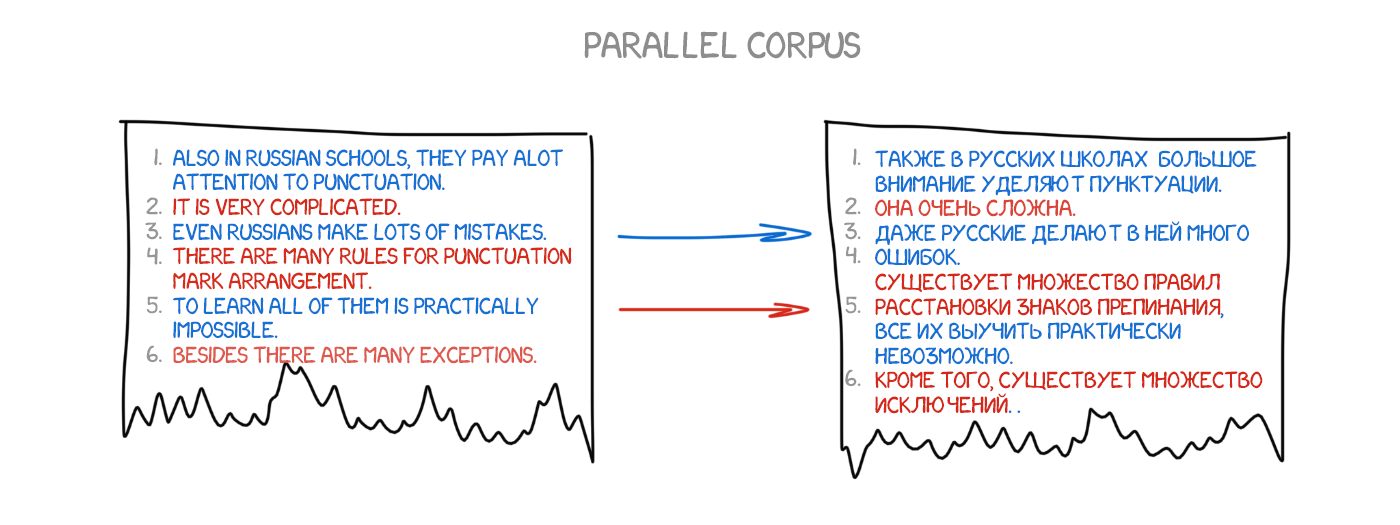
\includegraphics[width=\textwidth]{smt}
	\caption[Ví dụ về tập các câu song song trong hai ngôn ngữ]{Ví dụ về tập các câu song song trong hai ngôn ngữ: tiếng Anh - tiếng Nga, nguồn ảnh: Ilya Pestov trong blog \href{https://medium.freecodecamp.org/a-history-of-machine-translation-from-the-cold-war-to-deep-learning-f1d335ce8b5}{"A history of machine translation from the Cold War to deep learning"} }
	\label{fig_parallelcorpus}
\end{figure}

Mặc dù trên thực tế đã có nhiều hệ thống dịch máy được phát triển dựa trên dịch máy thống kê thời bấy giờ, tuy nhiên nó không hoạt động thực sự tốt bởi một số nguyên nhân. Một là việc những từ hay đoạn được dịch cục bộ và quan hệ của chúng với những từ cách xa trong câu nguồn thường bị bỏ qua. Hai là mô hình ngôn ngữ \textit{n}-gram hoạt động không thực sự tốt đối với những bản dịch dài và ta phải tốn nhiều bộ nhớ để lưu trữ chúng. Ngoài ra việc sử dụng nhiều thành phần nhỏ được điều chỉnh riêng biệt như mô hình dịch, mô hình ngôn ngữ, ... cũng gây khó khăn cho việc vận hành và phát triển mô hình này.

% TODO: Kalchbrenner and Blunsom (2013), Sutskever et al. (2014) and Cho et al. (2014b)
\textit{Dịch máy nơ-ron} (Neural machine translation) là một hướng tiếp cận mới cho bài toán dịch máy trong những năm gần đây và được đề xuất đầu tiên bởi \cite{kalchbrennerBlunsom}, \cite{Seq2Seq2014}, \cite{cho}. Giống như dịch máy thống kê, dịch máy nơ-ron cũng là một phương pháp thuộc hướng tiếp cận dựa trên ngữ liệu, trong khi dịch máy thống kê bao gồm nhiều mô-đun nhỏ được điều chỉnh riêng biệt, dịch máy nơ-ron cố gắng dùng một mạng nơ-ron như là thành phần duy nhất của hệ thống, mọi thiết lập sẽ được thực hiện trên mạng này. 

% TODO: Sutskever et al., 2014; Cho et al., 2014a
Hầu hết những mô hình dịch máy nơ-ron đều dựa trên kiến trúc \textit{Bộ mã hóa - Bộ giải mã} (Encoder-Decoder) (\cite{Seq2Seq2014}, \cite{cho}). Bộ mã hóa thường là một mạng nơ-ron có tác dụng \textit{"nén"} tất cả thông tin của câu trong ngôn ngữ nguồn vào một véc-tơ có kích thước cố định. Bộ giải mã, cũng là một mạng nơ-ron, sẽ tạo bản dịch trong ngôn ngữ đích từ véc-tơ có kích thước cố định kia. Toàn bộ hệ thống bao gồm bộ mã hóa và bộ giải mã sẽ được huấn luyện \textit{"end-to-end"}, quá trình này được mô tả như hình \ref{fig_encoder_decoder}.

\begin{figure}
	\centering
	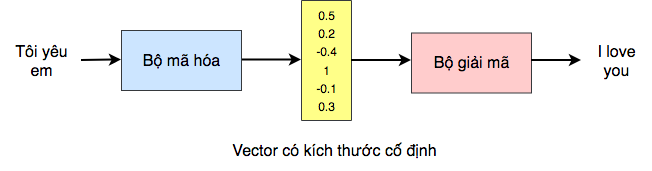
\includegraphics[width=\textwidth]{intro2nmt}
	\caption[Ví dụ về Kiến trúc \textit{Bộ mã hóa - Bộ giải mã} trong dịch máy nơ-ron]{Ví dụ về kiến trúc Bộ mã hóa - Bộ giải mã trong dịch máy nơ-ron}
	\label{fig_encoder_decoder}
\end{figure}

% TODO: mention LSTM
Trong thực tế cả bộ mã hóa và giải mã thường dựa trên một mô hình mạng nơ-ron tên là \textit{mạng nơ-ron hồi quy}; đây là một thiết kế mạng đặc trưng cho việc xử lý dữ liệu chuỗi. Mạng nơ-ron hồi quy cho phép chúng ta mô hình hóa những dữ liệu có độ dài không xác định, rất thích hợp cho bài toán dịch máy. Hình \ref{fig_encoder_decoder_details} mô tả chi tiết hơn về kiến trúc Bộ mã hóa - Bộ giải mã sử dụng mạng nơ-ron hồi quy. Đầu tiên mạng nơ ron hồi quy mà đóng vai trò bộ mã hóa sẽ duyệt qua từng từ trong câu nguồn, duyệt đến đâu sẽ cập nhật véc-tơ trạng thái ẩn (véc-tơ lưu thông tin cần thiết) của mạng đến đó, véc-tơ trạng thái ẩn cuối cùng được xem là chứa toàn bộ thông tin của câu nguồn được gọi là véc-tơ mã hóa của câu nguồn (véc-tơ này có kích thước cố định với các câu nguồn có chiều dài khác nhau). Véc-tơ mã hóa này sẽ được đưa vào một mạng nơ-ron hồi quy khác mà đóng vai trò là bộ giải mã. Tại một thời điểm, bộ giải mã sẽ phát sinh ra (hay giải mã ra) một từ trong câu đích dựa vào véc-tơ mã hóa câu nguồn và các từ đã sinh ra trước đó của câu đích.
\begin{figure}
	\centering
	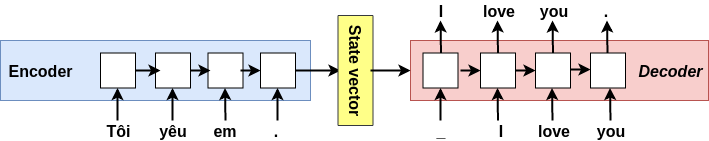
\includegraphics[width=\textwidth]{encoder-decoder}
	\caption[Kiến trúc Bộ mã hóa - Bộ giải mã được xây dựng trên mạng nơ-ron hồi quy]{Kiến trúc Bộ mã hóa - Bộ giải mã được xây dựng trên mạng nơ-ron hồi quy}
	\label{fig_encoder_decoder_details}
\end{figure}

Trong hình \ref{fig_encoder_decoder_details}, có thể thấy rằng bộ giải mã tạo ra bản dịch chỉ dựa trên trạng thái ẩn cuối cùng, cũng chính là véc-tơ có kích thước cố định được tạo ra ở bộ mã hóa. Véc-tơ này phải mã hóa mọi thứ chúng ta cần biết về câu nguồn. Giả sử chúng ta có câu nguồn với độ dài là 50 từ, từ đầu tiên ở câu đích có lẽ sẽ có mối tương quan cao với từ đầu tiên ở câu nguồn. Điều này có nghĩa là bộ giải mã phải xem xét thông tin được mã hóa từ 50 thời điểm trước đó. Mạng nơ-ron hồi quy được chứng minh là gặp khó khăn trong việc mã hóa những chuỗi dài \cite{pascanu2011}. Để giải quyết vấn đề này, thay vì dùng mạng nơ-ron hồi quy thuần, người ta sử dụng các biến thể của nó như \textit{Long short-term memory (LSTM)}. Trên lý thuyết, LSTM có thể giải quyết vấn đề mất mát thông tin trong chuỗi dài, nhưng trong thực tế vấn đề này vẫn chưa thể được giải quyết hoàn toàn. Một số nhà nghiên cứu đã phát hiện ra rằng đảo ngược chuỗi nguồn trước khi đưa vào bộ mã hóa tạo ra kết quả tốt hơn một cách đáng kể \cite{Seq2Seq2014} bởi nó khiến cho những từ đầu tiên được đưa vào bộ mã hóa sau cùng, và được giải mã thành từ tương ứng ngay sau đó. Cách làm này tuy giúp cho bản dịch hoạt động tốt hơn trong thực tế, nhưng nó không phải là một giải pháp về mặt thuật toán. Hầu hết các đánh giá về dịch máy được thực hiện trên các ngôn ngữ như ngôn ngữ có trật tự câu tương đối giống nhau. Ví dụ trật tự dạng "chủ ngữ - động từ - vị ngữ" như tiếng Anh, Đức, Pháp hay Trung Quốc. Đối với dạng ngôn ngữ có một trật tự khác ví dụ "chủ ngữ - vị ngữ - động từ" như tiếng Nhật, đảo ngược câu nguồn sẽ không hiệu quả.

Năm 2015, trong bài báo "Effective Apporoaches to Attention-based Neural Machine Translation" \cite{attentionThangLuong2015} được công bố tại hội nghị EMNLP, nhóm tác giả của Đại học Stanford (Minh-Thang Luong, Hieu Pham, Christopher D. Manning) đã đưa ra mô hình dịch máy LSTM-attention, trong đó đưa thêm cơ chế attention vào kiến trúc bộ mã hóa – bộ giải mã (ở đây, bộ mã hóa là một LSTM, bộ giải mã cũng là một LSTM). Cơ chế attention dựa trên quan sát rằng: tại một thời điểm trong quá trình giải mã, để quyết định từ tiếp theo của câu đích là gì thì không cần hết tất cả thông tin của câu nguồn mà chỉ cần thông tin của một số từ trong câu nguồn, nên chỉ cần tập trung (attend) vào một số từ trong câu nguồn. Như vậy, thay vì cố gắng mã hóa tất cả thông tin của câu nguồn vào trong véc-tơ mã hóa có kích thước cố định (điều mà khó thực hiện khi câu nguồn dài) và luôn dùng véc-tơ mã hóa này ở tất cả các thời điểm trong quá trình giải mã (điều mà không cần thiết), cơ chế attention cho phép ở mỗi thời điểm trong quá trình giải mã chỉ tập trung vào một vùng cần thiết trong câu nguồn (ở đây, một vùng nghĩa là một vài trạng thái ẩn trong tập tất cả các trạng thái ẩn của bộ mã hóa).

%\begin{figure}
%	\centering
%	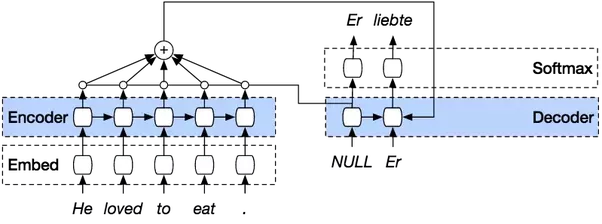
\includegraphics[width=\textwidth]{intro2attention}
%	\caption[Cơ chế Attention trong dịch máy nơ-ron]{Cơ chế Attention trong dịch máy nơ-ron}
%	\label{fig_introattention}
%\end{figure}

%Cơ chế Attention được miêu tả trong hình \ref{fig_introattention}. Ở đây tại mỗi bước tạo ra từ mới, bộ giải mã kết hợp trạng thái ẩn ở bước giải mã trước đó với một véc-tơ gọi là \textit{véc-tơ ngữ cảnh} để sinh ra trạng thái ẩn ở thời điểm hiện tại. Véc-tơ ngữ cảnh này là \textit{tổng có trọng số} của tất cả các véc-tơ trạng thái ẩn trong lúc mã hóa (đang đề cập đến \textit{global attention}). Với cách tiếp cận này, bộ giải mã không chỉ tạo ra bản dịch dựa trên véc-tơ mã hóa của câu nguồn mà còn tận dụng được cả những trạng thái ẩn ở câu nguồn trong quá trình mã hóa. Điều này giúp cho mô hình dịch máy trở nên hiệu quả hơn. Bên cạnh đó các trọng số tạo nên véc-tơ ngữ cảnh cho biết những từ trong câu đích đã "chú ý" đến những từ nào trong câu nguồn. Việc này giúp chúng ta phần nào giải thích được các kết quả của dịch máy nơ-ron - vốn rất khó giải thích vì tính phức tạp của nó.

Với những ưu điểm đã được trình bày của phương pháp dịch máy nơ-ron so với các phương pháp trước đó, cũng như là với những lợi ích khi sử dụng cơ chế attention trong dịch máy nơ-ron, trong khóa luận này chúng tôi tìm hiểu về mô hình dịch máy LSTM-attention được đề xuất trong bài báo “Effective Approaches to Attention-based Neural Machine Translation” \cite{attentionThangLuong2015} đã nói ở trên. Trong khóa luận này, chúng tôi đã thành công xây dựng lại mô hình được đề xuất trong bài báo. Bên cạnh đó chúng tôi cũng thực nhiều những thí nghiệm để kiểm tra độ hiệu quả của mô hình. Những thí nghiệm đó bao gồm: thí nghiệm so sánh giữa mô hình dịch máy nơ-ron sử dụng và không sử dụng attention và các thí nghiệm so sánh giữa các mô hình attention với nhau.

Các phần còn lại trong khóa luận được trình bày như sau:
\begin{itemize}
	\item[•] Chương 2 trình bày về những thành nền tảng của kiến trúc Bộ mã hóa - Bộ giải mã.
	
	\item[•] Chương 3 trình bày về cơ chế Attention, đây là phần chính của luận văn. Trong phần này gồm có hai phần nhỏ:
		\begin{itemize}
			\item[-] \textit{Global attetion}: là cơ chế tập trung vào tất cả các trạng thái ở câu nguồn
			\item[-] \textit{Local attetion}: tập trung vào một tập các trạng thái ở câu nguồn tại một thời điểm
		\end{itemize}
	\item[•] Chương 4 trình bày về các thí nghiệm và các phân tích về kết quả đạt trên hai tập dữ liệu Anh-Đức, Anh-Việt.
	\item[•] Cuối cùng, kết luận và hướng phát triển được trình bày ở chương 5.
\end{itemize}





